% siminos/presentations/spatiotemp/spatiotemp.tex        spatiotemp GTMAP18
% $Author: predrag $ $Date: 2021-12-06 16:21:14 -0500 (Mon, 06 Dec 2021) $

% remember to update \date{December 6, 2021}

%  started with siminos/presentations/GTMAP18/GTMAP18.tex   2018-04-13
%  started with siminos/presentations/GTmath18/GTmath18.tex 2018-02-24
%  started with siminos/presentations/KITP17/UCSB17.tex     2017-01-26
%  started with siminos/presentations/Israel16/Israel16.tex 2016-08-17
%  started with siminos/presentations/GTmap16/GTmap16.tex   2016-08-17
%  started with talks/predrag/NBI16/NBI16.tex               2016-04-25
%  started with talks/predrag/RoySoc16/RoySoc16.tex         2016-04-25

\input ../../inputs/layoutBeamer
\usepackage[font=scriptsize, labelfont=bf]{caption}
\usepackage[
    backend=biber,  %bibtex,
    sorting=nyt,
    %refsection=chapter,
    %citereset=chapter,
    style=numeric, %alphabetic, % %style=authoryear,
    natbib=true,
    style=phys, % aps
    biblabel= brackets, % superscript, %
    articletitle=false, % true,  % false, % aps
    %chaptertitle=true,  % aip;  % false, % aps
    pageranges = true , % aip: the full range
             % = false, % aps: only the first page being printed
    sortlocale=en_US,
    giveninits=true,
    url=false, %true,  %
    doi=false, %true,
    eprint=false
]{biblatex}
\addbibresource{../../bibtex/siminos.bib}
\setbeamerfont{footnote}{size=\tiny}
\input{../../inputs/def} % no edits, always from dasbuch/book/inputs
\input{../../inputs/defsBeamer}
\renewcommand{\Ssym}[1]{{\ensuremath{m_{#1}}}}    % Boris
% \newcommand{\Ssym}[1]{{\ensuremath{s_{#1}}}}  % ChaosBook

% temporary fix, will not be needed in later MixTeX version         2018-11-02
% https://tex.stackexchange.com/questions/426088/texlive-pretest-2018-beamer-and-subfig-collide
\makeatletter
\let\@@magyar@captionfix\relax
\makeatother

\begin{document}


\title{
{a spatiotemporal theory of}
{\huge turbulence}
    \\
{computational challenges}
}
\author{P. Cvitanovi\'c}
\author[Cvitanovi\'c]
{
  \textcolor{green!50!black}{
  {Predrag~Cvitanovi\'c
  and
  Matt Gudorf
  }	%\inst{1}
  }
}
\institute
{
%  \inst{1}%
working notes
\\
                Georgia Tech
 }
\date{December 6, 2021}
    %{October 9, 2020}
    %{May 25, 2019}
    %{March 30, 2019}
    %{November 29, 2018}
    %{April 27, 2018}

\begin{frame}{}
%\begin{center}
\hfill\includegraphics[width=0.55\textwidth]{HoweyCats}
%\end{center}
\end{frame}


\begin{frame}
  \titlepage
\end{frame}


\section[what this work is about]
 {what this work is about}

\begin{frame}{overview}
\begin{enumerate}
              \item {\Large
what this talk is about
                  }\textcolor{gray}{\small
              \item
turbulence in large domains
              \item
space is time
              \item
bye bye, dynamics
                    }
            \end{enumerate}
\end{frame}

\begin{frame}{how do clouds solve PDEs?}

\vfill

do clouds \textcolor{red}{integrate} Navier-Stokes equations?

\begin{center}
\centerline{\textcolor{red}{\Huge ?}}
%\end{center}
%for weather prediction, we store sets of weather sequences
%\bigskip\bigskip

%\begin{center}
\begin{minipage}[t]{\textwidth}
	\begin{center}
%\vspace{2ex}
\centerline{
\raisebox{-4.0ex}[5.5ex][4.5ex]
		 {\includegraphics[height=12ex]{Hopf-a}}
~~~ $\Longrightarrow$ ~~ {other swirls} ~~ $\Longrightarrow$ ~~~
	\raisebox{-4.0ex}[5.5ex][4.5ex]
		 {\includegraphics[height=12ex]{Hopf-b}}
          }
	\end{center}
\end{minipage}
\end{center}

are clouds Navier-Stokes supercomputers in the sky?

\end{frame}

\begin{frame}{part 1}
\begin{enumerate}
              \item {\Large
turbulence in large domains
                  }\textcolor{gray}{\small
              \item
space is time
              \item
spacetime
              \item
bye bye, dynamics
                    }
            \end{enumerate}
\end{frame}


\begin{frame}{goal : enumerate the building blocks of turbulence}
\begin{block}{Navier-Stokes equations} % (1822)}
\[
\dfrac{\partial \bv}{\partial t} + (\bv \cdot \nabla) \bv
	\,=\,
\frac{1}{R} \nabla ^2 \bv
-\nabla p
+ \mathbf{f}
    \,,\qquad
\nabla \cdot \bv = 0,
\]
\end{block}

\hfill{\small
velocity field  $\bv \in \mathbb{R}^3$
;
pressure field $p$
;
driving force $\mathbf{f}$
        }

\medskip

\begin{block}{describe turbulence}
starting from the equations (no statistical assumptions)
\end{block}

\bigskip

% large Reynolds number $R$:
\hfill {\Large\textcolor{red}{}}

\end{frame}

\begin{frame}{challenge : experiments are amazing}
\begin{center}
\includegraphics[width=0.7\textwidth]{mullin_puff2200} %pipe}
\end{center}
T. Mullin lab
\begin{center}
\bigskip
\includegraphics[width=0.7\textwidth]{deLHof09fig6} %pipe}
\end{center}
B. Hof lab
\end{frame}

%\begin{frame}{pipe theory and numerics}
%	\begin{columns}[t]
%	\column{.55\textwidth}
%amazing experiments! \\ amazing numerics! \\ beautiful visualizations !
%
%\bigskip\bigskip
%
%%relative periodic orbits,
%``Exact Coherent Structures'' :
%\\ numerical Navier-Stokes
%
%\medskip
%isosurfaces and cross sections \\ of the streamwise velocity
%
%\medskip
%
%\textcolor{red}{red} (\textcolor{blue}{blue}) streaks
%\\ are \textcolor{red}{faster} (\textcolor{blue}{slower}) \\ than the base flow
%
%\bigskip
%
%{{\tiny Ritter et al., Phys. Rev. Fluids (2018)}}
%
%	\column{.45\textwidth}
%\begin{center}
%  \includegraphics[width=1.0\textwidth,clip=true]
%                    {RZSEA18Fig3}
%\end{center}
%	\end{columns}
%\end{frame}

\section[dynamics in $\infty$ dimensions]
{dynamics in $\infty$ dimensions}

\begin{frame}{can simulate {\Huge large} computational domains}
\begin{center}
\includegraphics[width=1.0\textwidth]{AviHof13fig4}
\end{center}
pipe flow close to onset of turbulence
\footnote{M.~Avila and B.~Hof, {Phys. Rev. \bf E 87} (2013)}

\bigskip

but we have \textcolor{red}{\Huge hit a wall} :

\hfill exact coherent structures are too unstable to compute
\end{frame}

\begin{frame}{goal : we can do 3D turbulence, but for this presentation}
\begin{block}{Navier-Stokes equations} % (1822)}
\[
\dfrac{\partial \bv}{\partial t} + (\bv \cdot \nabla) \bv
	\,=\,
\frac{1}{R} \nabla ^2 \bv + (\cdots)
% -\nabla p + \mathbf{f}
%    \,,\qquad
%\nabla \cdot \bv = 0,
\]
\end{block}

\hfill{\small velocity field  $\bv(\bx;t) \in \mathbb{R}^3$}

\medskip

\begin{block}{not helpful for developing intuition}
we cannot visualize 3D velocity field at every 3D spatial point
\end{block}

\bigskip

% large Reynolds number $R$:
\hfill {\Large\textcolor{red}{look instead at 1D `flame fronts'}}
\end{frame}

\begin{frame}{(1+1) spacetime dimensional ``Navier-Stokes''}
\begin{block}{Navier-Stokes equations \hfill (1822)}
\[
\dfrac{\partial \bv}{\partial t} + (\bv \cdot \nabla) \bv
	\,=\,
\frac{1}{R} \nabla ^2 \bv + (\cdots)
\]
\end{block}
    \centerline{\textcolor{red}{$\blacktriangledown$}}
    \centerline{\textcolor{red}{$\blacktriangledown$}}
    \centerline{\textcolor{red}{$\blacktriangledown$}}
\begin{block}{\KS\ (1+1)\dmn\ PDE \hfill (1975)}
\[
  u_t + u \triangledown u \,=\,
    {\color{red}-}\triangledown^2 u {\color{red}-\triangledown^4 u}
    \,,\qquad   x \in \mathbb{R}
    \,,
\]
\end{block}
\bigskip

describes spatially extended systems such as
\begin{itemize}
 \item flame fronts in combustion
 \item reaction-diffusion systems
 \item \ldots
\end{itemize}
\end{frame}

\begin{frame}{an example : \KS\ on a large domain}
\begin{center}
  \includegraphics[width=.6\textwidth]{MNG_uu500b500}
%  \includegraphics[width=0.6\textwidth] %,height=0.5\textheight,clip=true]
%  {ks_largeL_cbar_200} %{ksevol-fig} %{ks_largeL_cbar}
\end{center}

{\footnotesize
[horizontal] space $\ssp \in [0,L]$
\qquad
{[up]} time evolution
}

\begin{itemize}
\item turbulent behavior
\item simpler physical, mathematical and computational setting than Navier-Stokes
\end{itemize}
\end{frame}

\begin{frame}{another example of large spacetime domain simulation}
\begin{block}{complex Ginzburg-Landau}
  \includegraphics[width=0.515\textwidth] %,height=0.5\textheight,clip=true]
  {cGLdefturbabs}
  \hfill
  (will return to this)
\end{block}

{\footnotesize
[horizontal] space $\ssp \in [-L/2,L/2]$
\qquad
{[up]} time evolution
}

\hfill {\scriptsize \color{orange} codeinthehole.com/static/tutorial/coherent.html}
\end{frame}

\begin{frame}{compact space, infinite time cylinder}
\begin{center}
\includegraphics[width=0.9\textwidth]{cylinderTime}
\end{center}
% \hfill \color{red}{(impossible without xxx)}
so far : Navier-Stokes on compact spatial domains, all times
\end{frame}

\begin{frame}{compact space, infinite time} % \KS}
\begin{block}{\KS\ equation}
\[
  u_t \,=\,
    -({\color{red}+}\triangledown^2 +{\color{red}\triangledown^4}) u
    - u \triangledown u
    \,,\qquad   x \in [-L/2,L/2]
    \,,
\]
\end{block}

\bigskip

\begin{block}{in terms of discrete spatial Fourier modes}
$N$ ordinary differential equations (ODEs) in time
\[
\dot{\Fu}_k(\zeit) = ( q_k^2 - q_k^4 )\, \Fu_k(\zeit)
- i \frac{q_k}{2} \!\sum_{k'=0}^{N-1} \!\!\Fu_{k'}(\zeit) \Fu_{k-k'}(\zeit)
\,.
%\label{e-Fks}
\]
\end{block}
\end{frame}


\subsection{types of solutions}
\begin{frame}{evolution of \KS\ on small $L=22$ cell}
\begin{center}
  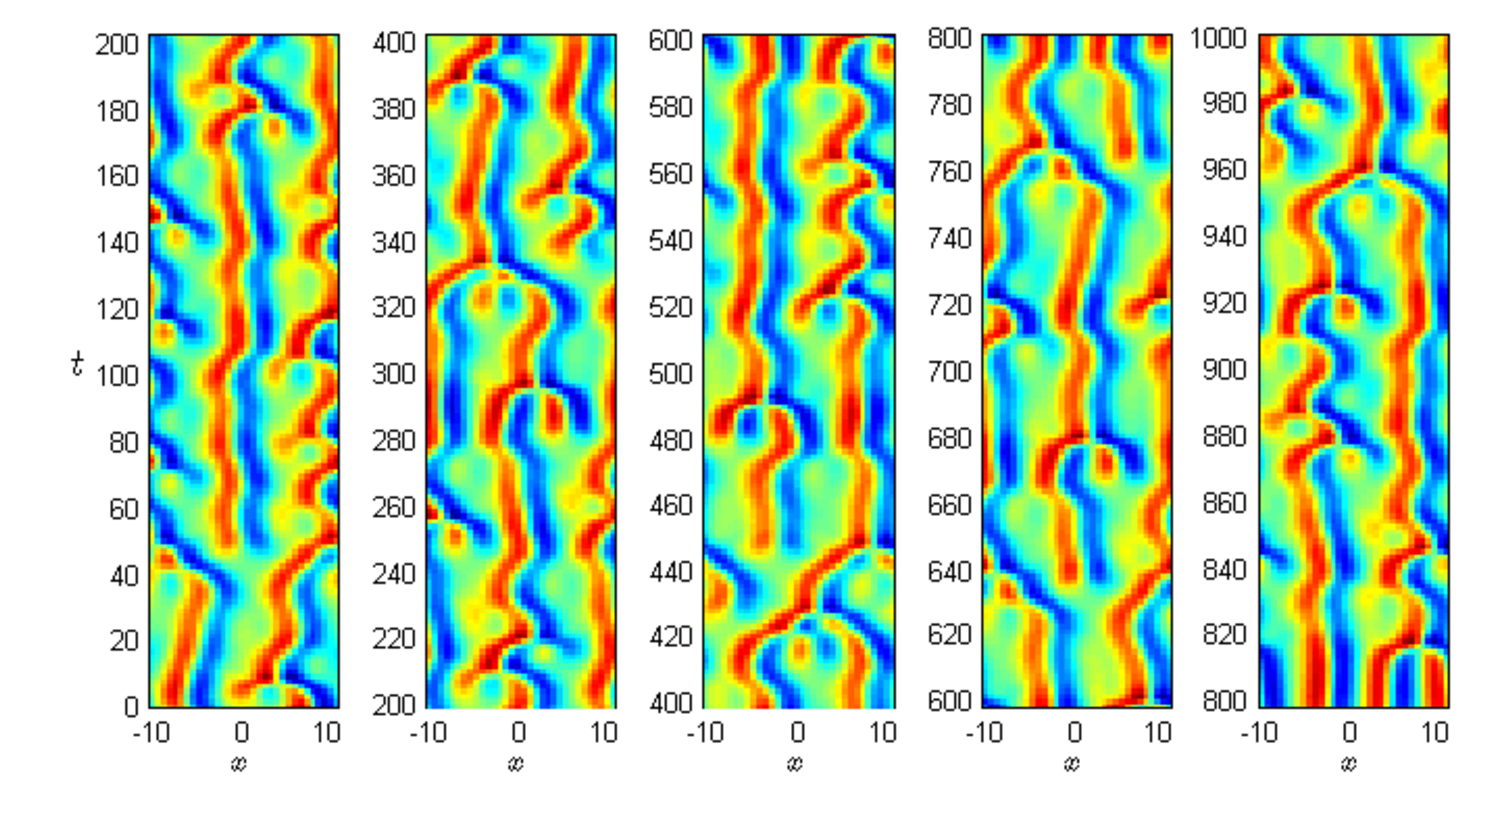
\includegraphics[width=0.9\textwidth,clip=true]{ks_L22_long_orbit}
\end{center}
horizontal: $x \in [-11,11]$
\\
vertical: time
\\
color: magnitude of $u(x,t)$
\end{frame}

\begin{frame}{part 2}
\begin{enumerate}
              \item
    \textcolor{gray}{\small
turbulence in large domains
        }
              \item
    {\Large
space is time
    }\textcolor{gray}{\small
              \item
spacetime
              \item
bye bye, dynamics
                    }
            \end{enumerate}
\end{frame}

\begin{frame}{yes, but}
\begin{center}
{\huge is space time?}
\end{center}
\end{frame}

\begin{frame}{compact time, infinite space}
rewrite \KS
\bea
    u_\zeit &=&  - u u_\conf
    -u_{\conf \conf}-u_{\conf \conf \conf \conf}
\nonumber     % \label{e-ks}
\eea
 as  4-fields vector
\bea
\transp{{\bf u}}&=&(u,u^{'},u^{''},u^{'''})
    \continue
&& \mbox{where }
    u^{'}   \equiv u_{\conf} \,,\;
    u^{''}  \equiv u_{\conf \conf} \,,\;
    u^{'''} \equiv u_{\conf \conf \conf}
\nnu
\eea
equation
\(
\frac{d~}{d\conf}{\bf u}(x)={\bf v}(x)
\)
now {\color{blue}1st order} in {\color{blue}spatial} derivative
\begin{block}{\KS\ = four coupled 1st order PDEs}
\bea
    \frac{d\,u}{d\conf}       &=& u^{'}
\,,\qquad
    \frac{d\,u^{'}}{d\conf}   \,=\,   u^{''}
\continue
    \frac{d\,u^{''}}{d\conf~}   &=&   u^{'''}
\,,\qquad
    \frac{d\,u^{'''}}{d\conf~~}  \,=\,  - u_{\zeit} - u^{''} - u\,u^{'}
\nonumber
\eea
\end{block}
\end{frame}

\begin{frame}{compact time, infinite space}
  1st order in {\color{blue}spatial} derivative
\begin{block}{evolve four 1st order PDEs for ${\bf u}(x)$ in $\conf$,}
\begin{itemize}
  \item
\[
\frac{d~}{d\conf}{\bf u}(x)={\bf v}(x)
\]
  \item
compact in time, periodic boundary condition
\[
  u(\conf, \zeit) = u(\conf, \zeit + \period{})
\]
  \item
initial data
\[
  \transp{{\bf u}}_0=(u(\conf_0, \zeit),u^{'}( \conf_0, \zeit),
                      u^{''}( \conf_0, \zeit),u^{''}( \conf_0, \zeit))
\]
specified for all $\zeit \in [0, \period{})$, at a fixed space point $\conf_0$
\end{itemize}
\end{block}
\end{frame}

\begin{frame}{can do : compact time, infinite space cylinder}
\begin{center}
\includegraphics[width=0.9\textwidth]{cylinderSpace}
\end{center}
% \hfill \color{red}{(impossible without xxx)}
\end{frame}

\begin{frame}{a time-invariant \eqv, spatial \po}
\begin{center}
  \begin{minipage}[height=.45\textheight]{.45\textwidth}
    \centering \small{\texttt{(left)}}
    \includegraphics[width=\textwidth,height=.45\textheight]{MNGeq1time}
  \end{minipage}
  \begin{minipage}[height=.45\textheight]{.45\textwidth}
    \centering \small{\texttt{(right)}}
    \includegraphics[width=\textwidth,height=.45\textheight]{MNGeq1space}
  \end{minipage}
\end{center}
   %\caption{
  evolution of $\EQV{1}$ : (left) in time, (right) in space
   \\
   initial condition for the spatial integration is the time strip
   $u(\conf_0,\zeit)$, $\zeit = [0,\period{})$, where time period
   $\period{} =0$, spatial $x$ period is $L=22$.
   % }\label{fig:MNGeqva1spttmp}

\vfill\hfill        Michelson 1986
%, Gudorf 2016
\end{frame}

\begin{frame}{a spacetime \twot\ integrated in either time or space}
\begin{center}
  \begin{minipage}[height=.40\textheight]{.35\textwidth}
    \centering \small{\texttt{(left)}}
    \includegraphics[width=\textwidth,height=.60\textheight]{MNGcomp32xint22}
  \end{minipage}
~~~~~~~~~
  \begin{minipage}[height=.40\textheight]{.35\textwidth}
    \centering \small{\texttt{(right)}}
    \includegraphics[width=\textwidth,height=.60\textheight]{MNGcomp64xint22}
  \end{minipage}
\end{center}
    (left) old : time evolution. (right) new : space evolution
    \\
    $x=[0,L]$ %22]$,
       initial condition : time periodic line $t = [0,T]$
  %2\,T_{\PPO{10.2}})$
  %\label{fig:MNGcompxint2}

\vfill\hfill        Gudorf 2016
\end{frame}

\begin{frame}{but integrations are uncontrollably unstable}

\begin{center}
{\huge neither} time {\huge nor} space integration {\huge works} \\
for large domains
\end{center}

\vfill
\color{red}{rethink the calculation}
\end{frame}

%%%%%%%%%%%%%%%%%%%%%%%%%%%%%%%%%%%%%%%%%%%%%%%%%%%%%%%%%%%%%%%%%%%%%%%%%%%
\begin{frame}{part 3}
\begin{enumerate}
              \item
    \textcolor{gray}{\small
turbulence in large domains
              \item
space is time
    }
              \item {\Large
spacetime
    }\textcolor{gray}{\small
              \item
bye bye, dynamics
                    }
            \end{enumerate}
\end{frame}

\begin{frame}{complex Ginzburg-Landau on a large spacetime domain}
\begin{block}{goal : enumerate nearly recurrent chronotopes}
  \includegraphics[width=0.4635\textwidth]{cGLdefturbabs}%
~~\raisebox{+3.33ex}[5.5ex][4.5ex]
		 {\includegraphics[width=0.36\textwidth]{cGLdefturbclip}}
\end{block}

{\footnotesize
[left-right] space $\ssp \in [-L/2,L/2]$
\qquad
{[up]} time $t\in [0,\period{}]$
}
\end{frame}

\begin{frame}
    \frametitle{\KS\ on a large spacetime domain}
\begin{block}{the same small tile recurs often in a turbulent pattern}
\includegraphics[width=.48\textwidth]{MNG_uu500b500co}
\includegraphics[width=.48\textwidth]{cutouts}
\end{block}
goal : define, enumerate nearly recurrent tiles
\end{frame}

\begin{frame}{chronotope
    \footfullcite{LePoTo96}%$^,$\footfullcite{WK09}
}
\begin{bartlett}{
In literary theory and philosophy of language, the chronotope is how
configurations of time and space are represented in language and
discourse.
                }\bauthor{
\HREF{https://en.wikipedia.org/wiki/Chronotope}
{Wikipedia : Chronotope}
                }
\end{bartlett}

\bigskip
\bigskip
%goes without saying : was done by a Soviet scientist first

\begin{itemize}
  \item Mikhail Mikhailovich Bakhtin (1937)
%  \item Politi, Giacomelli, Lepri, Torcini (1996)
%  \item Gutkin and Osipov (2016)
\end{itemize}
\end{frame}

\begin{frame}{use spatiotemporally compact solutions as chronotopes}
\begin{center}
\includegraphics[width=0.9\textwidth]{torusSpTime}
\end{center}
this `exact coherent structure'\\
\textcolor{red}{shadows} a small patch of spacetime solution $u( \conf, \zeit)$
\end{frame}

\begin{frame}{\po s generalize to $d$-tori}

\begin{block}{1 time, 0 space dimensions}
a {\statesp} point is {\em periodic} if its orbit returns to it
after a finite time \period{} ;
\\
such orbit tiles the time axis
by infinitely many repeats
\end{block}

\bigskip

\begin{block}{1 time, $d$-1 space dimensions}
 a {\statesp} point is {\em spatiotemporally periodic} if
it belongs to \\ an invariant $d$-torus ${\R}$ ;
\\
such torus tiles the spacetime
by infinitely many repeats
%,\\
%\ie, a \brick\ $\Mm_{\R}$ that
%tiles the lattice state  $\Mm$, \\
%with period $\ell_j$ in $j$th lattice direction
\end{block}
\end{frame}

\begin{frame}{a spacetime \twot\ integrated in either time or space}
\begin{center}
  \begin{minipage}[height=.40\textheight]{.35\textwidth}
    \centering \small{\texttt{(left)}}
    \includegraphics[width=\textwidth,height=.60\textheight]{MNGcomp32xint22}
  \end{minipage}
~~~~~~~~~
  \begin{minipage}[height=.40\textheight]{.35\textwidth}
    \centering \small{\texttt{(right)}}
    \includegraphics[width=\textwidth,height=.60\textheight]{MNGcomp64xint22}
  \end{minipage}
\end{center}
    (left) ~~~old : time evolution
    ~~~~~$t=[0,\period{}]$ %22]$,
        \\ \hfill {\scriptsize
       initial condition : space periodic line $x = [0,\speriod{}]$
                  }
        \\
    (right) new : space evolution
    $x = [0,\speriod{}]$ %22]$,
        \\ \hfill {\scriptsize
       initial condition : time periodic line $t = [0,\period{}]$
                  }
  %2\,T_{\PPO{10.2}})$
  %\label{fig:MNGcompxint2}

\vfill\hfill        Gudorf 2016
\end{frame}

\begin{frame}{every compact solution is a fixed point on a discrete lattice}
discretize $u_{nm} = u(\conf_n,\zeit_m)$ over
$N M$ points of spatiotemporal periodic lattice $\conf_n = n L/N$,
 $\zeit_m = m \period{}/M$, Fourier transform :
\[
\Fu_{k\ell} \,=\,
  \frac{1}{NM} \sum^{N-1}_{n=0} \sum^{M-1}_{m=0}
  u_{nm} \, e^{-i(q_k\conf_n + \omega_\ell \zeit_m)}
    \,,\quad
q_k = \frac{2 \pi k}{L}
    \,,\;
\omega_\ell = \frac{2 \pi \ell}{\period{}}
% \label{spattempFT}
\]
\KS\ is no more a PDE, \\
but an {\color{blue}{algebraic}} $[N\!\times\!M]$\dmn\ problem\\
of determining {\color{blue}{global}} solution ${\bf u}$ to
\begin{block}{fixed point condition}
\[
\left(- i \omega_\ell - ( q_k^2 - q_k^4 ) \right)\Fu_{k\ell}
+ i \frac{q_k}{2} \!\sum_{k'=0}^{N-1} \sum^{M-1}_{m'=0}\!\!
\Fu_{k'm'} \Fu_{k-k',m-m'}
    = 0
\]
\end{block}
\end{frame}

\begin{frame}{every calculation is a spatiotemporal lattice calculation}
field is discretized as
$\Fu_{k\ell}$ values  \\ over
$N M$ points of a periodic lattice

%\medskip

\begin{center}
\includegraphics[width=0.9\textwidth]{torusSpTime}
\end{center}
% \hfill \color{red}{(impossible without xxx)}
\end{frame}

\begin{frame}{professor Zweistein forgets to take his meds}
\medskip
statement : {\huge HA!} \\
You are imposing by hand the space \& time periods
\speriod{}, \period{} {\huge !}

\begin{center}
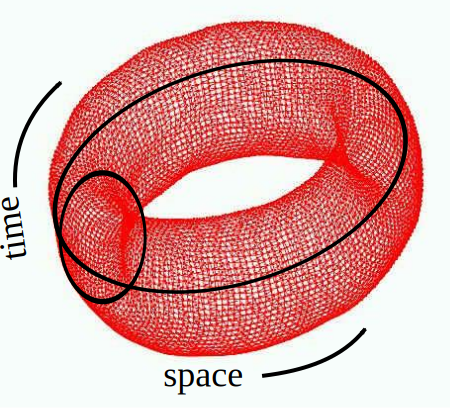
\includegraphics[width=0.35\textwidth]{spaceTime1}
\end{center}

answer : {\huge\color{red}{NO!}} \\
nature chooses \speriod{} \& \period{},
they are free parameters.
\end{frame}

\begin{frame}{there is no more time evolution}
solution to \KS\ is now given as
\begin{block}{condition that}
at each lattice point $k\ell$ \\
the tangent field at $\Fu_{k\ell}$
\end{block}
satisfies the equations of motion
\[
\left[- i \omega_\ell - ( q_k^2 - q_k^4 ) \right]\Fu_{k\ell}
+ i \frac{q_k}{2} \!\sum_{k'=0}^{N-1} \sum^{M-1}_{m'=0}\!\!
\Fu_{k'm'} \Fu_{k-k',m-m'}
    =
0
%\,.
%\label{e-FksSpattemp}
\]

\bigskip

this is a \textcolor{red}{local} tangent field constraint on a \textcolor{red}{global} solution
\end{frame}

\begin{frame}{think globally, act locally}
    \begin{center}
\includegraphics[width=0.85\textwidth]{globalLocal}
    \end{center}
for each symbol array \Mm, a periodic lattice state $\Xx_\Mm$
\end{frame}

\begin{frame}{unexpected gift from nature}
robust : no exponential instabilities
\\
\hfill as there are no finite time / space integrations
\bigskip

no need for $\sim
10^{-11}$ accuracies,
\bigskip

{\huge \textcolor{red}{so}}
\bigskip

accuracy to a few \% suffices, \\
\hfill you only need to get the shape of a solution right
\end{frame}

\begin{frame}{part 4}
\begin{enumerate}
              \item
    \textcolor{gray}{\small
turbulence in large domains
              \item
space is time
              \item
spacetime    }
              \item {\Large
spacetime computations
    }\textcolor{gray}{\small
              \item
bye bye, dynamics
                    }
            \end{enumerate}
\end{frame}


\begin{frame}{how to find solutions ? an ODE example}
\begin{center}
the law of motion : $\qquad \dot{\ssp} = \pVeloc(\ssp)$
\begin{minipage}[c]{0.55\textwidth}
\textcolor{red}{guess loop tangent}
$\lVeloc(\lSpace)
	\neq
\pVeloc(\lSpace)$

	\vskip 0.5cm

\textcolor{green}{periodic orbit}
$\lVeloc(\lSpace)$,~$\pVeloc(\lSpace)$
aligned
\end{minipage}%
~~~~~~~\begin{minipage}[c]{0.40\textwidth}
	\begin{center}
	\includegraphics[width=0.7\textwidth]{velocField}
	\end{center}
\end{minipage}
\end{center}
\begin{block}{cost function}%
\[
\costF[\lSpace] =
            \oint_\Loop ds\,(\lVeloc-\pVeloc)^2
    \,;\quad
    \lVeloc = \lVeloc(\lSpace(s,\tau))\,,\,\,
    \pVeloc = \pVeloc(\lSpace(s,\tau))
\,,
% \label{loopCostFct}
\]
\end{block}
\bigskip

penalize\footfullcite{lanVar1}%{ Lan and Cvitanovi\'c, Phys. Rev. (2004)}
 misorientation of the loop tangent
$\lVeloc(\lSpace)$
relative to the true dynamical flow tangent field $\pVeloc(\lSpace)$
\end{frame}

\begin{frame}{how do clouds solve PDEs?}
clouds do not \textcolor{red}{\Huge NOT} {integrate} Navier-Stokes equations

\bigskip\bigskip

\begin{center}
\begin{minipage}[t]{\textwidth}
	\begin{center}
\centerline{
\raisebox{-4.0ex}[5.5ex][4.5ex]
		 {\includegraphics[height=12ex]{Hopf-a}}
~~~ $\Longrightarrow$ ~~ {other swirls} ~~ $\Longrightarrow$ ~~~
	\raisebox{-4.0ex}[5.5ex][4.5ex]
		 {\includegraphics[height=12ex]{Hopf-b}}
          }
	\end{center}
\end{minipage}
\end{center}

do clouds satisfy Navier-Stokes equations?

\bigskip

{\Large yes!}

\centerline{
\textcolor{blue}{they satisfy them \textcolor{red}{\large locally}, everywhere and at all times}
}
\end{frame}

\begin{frame}{the equations imposed as local constraints}
\begin{block}{\KSe}
\[
F(u) = u_t + u_{\conf \conf} + u_{\conf \conf \conf \conf} + u u_{\conf} = 0
\]
\end{block}
\bigskip\bigskip
for example, minimize over the entire 2-torus
\begin{block}{cost function}
\[
G \equiv \frac{1}{2} |F(u)|^2_{L \times T}
%\ee{costfunctional}
\]
\end{block}
\vfill\hfill\textcolor{red}{\Huge need your help !}
\end{frame}

\begin{frame}{adjoint descent}
cost function
\[
  G = \frac{1}{2} \mathbf{F}^{\top}\mathbf{F}
  \,.
\]
introduce fictitious time ($\tau$) flow by differentiation of cost function.
\[
  \partial_{\tau}G = (J^{\top}\mathbf{F})^{\top}(\partial_{\tau}\mathbf{x})
\]
  ``adjoint descent'' method defined by chosing\footfullcite{Faraz15}
\[
  \partial_{\tau}\mathbf{x} = -(J^{\top}\mathbf{F})
\]

\end{frame}

\begin{frame}{does it work at all ?}
add strong noise to a \emph{known} solution, \\ twice the typical amplitude
\begin{block}{only the first test}
{\scriptsize (not how we actually generate guesses)} \\
\begin{minipage}[height=.32\textheight]{.35\textwidth}
\centering %\small{\texttt{(a)}}
\includegraphics[width=\textwidth,height=.32\textheight]{MNG_ppo1_noise_init}
\end{minipage}
    \qquad
\begin{minipage}[height=.32\textheight]{.35\textwidth}
\centering %\small{\texttt{(right)}}
\includegraphics[width=\textwidth,height=.32\textheight]{MNG_ppo1_noise_conv}
\end{minipage}
%\caption{ \label{fig:MNG_adjnewt_robustness}
\end{block}

{\scriptsize (left) initial guess: a known %\PPO{10.2}
\twot} \\
$(\speriod{0},\period{0})=(22.0,20.5057459345)$
+
strong random noise
\medskip

{\scriptsize (right) the resulting adjoint descent converged \twot} \\
$(\speriod{f},\period{f})=(21.95034935834641,20.47026321555662)$
%\end{figure}
\end{frame}

\begin{frame}{initial guess generation ?}
 \textcolor{blue}{the time scale} : the shortest
`turnover' scale characterized by the period of the shortest \po? Or perhaps
the Lyapunov time?

\bigskip

\textcolor{blue}{the spatial scale} :
$\bar{L}=2\pi\sqrt{2}$, the  most unstable spatial wavelength of the \KS

\bigskip

%%%%%%%%%%%%%%%%%%%%%%%%%%%%%%%%%%%%%%%%%%%%%%%%%%%%%%%%%%%%%%%%
%\label{fig:MNG_spacetime_smoothed} from siminos/spatiotemp/blogMNG.tex
\begin{minipage}[height=.32\textheight]{.30\textwidth}
\includegraphics[width=\textwidth,height=.32\textheight]{MNG_T100L44_init}
\end{minipage}

\medskip
initial : spatial $\bar{L}$-modulated random guess
%%%%%%%%%%%%%%%%%%%%%%%%%%%%%%%%%%%%%%%%%%%%%%%%%%%%%%%%%%%%%%%%

% \vfill\hfill        Gudorf 2018
\end{frame}

\begin{frame}{KS \twot\ found variationally}
%%%%%%%%%%%%%%%%%%%%%%%%%%%%%%%%%%%%%%%%%%%%%%%%%%%%%%%%%%%%%%%%
%\label{fig:MNG_spacetime_smoothed} from siminos/spatiotemp/blogMNG.tex
\begin{minipage}[height=.72\textheight]{.40\textwidth}
\centering \small{\texttt{(left)}}
\includegraphics[width=\textwidth,height=.63\textheight]{MNG_T100L44_init}
\end{minipage}
\begin{minipage}[height=.72\textheight]{.40\textwidth}
\centering \small{\texttt{(right)}}
\includegraphics[width=\textwidth,height=.63\textheight]{MNG_T100L44_final}
\end{minipage}

\vfill
(left) initial : $\bar{L}=2\pi\sqrt{2}$ spatially modulated ``noisy'' guess

(right) adjoint descent : converged \twot\
% \\
% spatial and time periods
% $L=24.07$, $T=31.86$
%%%%%%%%%%%%%%%%%%%%%%%%%%%%%%%%%%%%%%%%%%%%%%%%%%%%%%%%%%%%%%%%

\vfill\hfill        Gudorf 2018
\end{frame}


\begin{frame}{initial guesses, embedded in ergodic sea?}
\begin{block}{Historically, }
guesses extracted from close recurrences \\
observed in long turbulent simulations
\end{block}
\bigskip\bigskip
            \begin{enumerate}
              \item
inefficient, finds only the shortest, least unstable orbits%
\footfullcite{pchaot}$^,$\footfullcite{GHCW07}
              \item
can integrate only not far in time
            \end{enumerate}

\vfill\hfill\textcolor{red}{\huge need spatiotemporal guesses}
\end{frame}

\begin{frame}{guesses extracted from large spacetime domains}
\begin{minipage}[height=.45\textwidth]{.45\textwidth}
\centering %\small{\texttt{(a)}}
\includegraphics[width=\textwidth,height=.45\textheight]{MNGadjdescent500b500init}
\end{minipage}
\begin{minipage}[height=.45\textwidth]{.45\textwidth}
\centering %\small{\texttt{(b)}}
\includegraphics[width=\textwidth,height=.45\textheight]{MNGadjdescent500b500fin}
\end{minipage}
%\caption{ \label{fig:MNGlarge_adjointdescent}

(left) random initial state on
%\hfill
$(\speriod{},\period{})=(500,500)$

(right) adjoint descent $\to$ typical \KS\ state

\vfill\hfill
finite windows are our starting guesses for \twots
\end{frame}

\begin{frame}{another, much twittered : machine learning guesses}
``reservoir computing'' example\footfullcite{PHGLO18}

\bigskip

 \begin{columns}
 \column{0.35\textwidth}
~~~~~~\includegraphics[width=1\textwidth]{PHGLO18fig2}
 \column{0.65\textwidth}
 \begin{itemize}
 \item[(a)] data: \\ \KS\ simulation
 \item[(b)] reservoir computing prediction
 \item[(c)] two subtracted agree to \\
            $\sim 5$ Lyapunov times
 \end{itemize}
 \end{columns}
\vfill {\Large Q : \textcolor{red}{how would you learn this data?}}
\end{frame}

\begin{frame}{embarrassment of riches}
\begin{center}
{\huge what to do?}
\end{center}

\vfill

{\Large Matthew N. Gudorf}

\medskip

\hfill has 1\,000's of such \twots
\end{frame}


\begin{frame}{part 5}
\begin{enumerate}
              \item
    \textcolor{gray}{\small
turbulence in large domains
              \item
space is time
              \item
spacetime
    }
              \item {\Large
fundamental tiles
    }\textcolor{gray}{\small
              \item
bye bye, dynamics
                    }
            \end{enumerate}
\end{frame}


\begin{frame}{building blocks of turbulence}

how do we \textcolor{red}{recognize} a cloud?

\bigskip
\begin{center}
\centerline{\textcolor{red}{\Huge WATCH}}
%\end{center}
%for weather prediction, we store sets of weather sequences
%\bigskip\bigskip

%\begin{center}
\begin{minipage}[t]{\textwidth}
	\begin{center}
%\vspace{2ex}
\centerline{
\raisebox{-4.0ex}[5.5ex][4.5ex]
		 {\includegraphics[height=12ex]{Hopf-a}}
~~~ $\Longrightarrow$ ~~ {other swirls} ~~ $\Longrightarrow$ ~~~
	\raisebox{-4.0ex}[5.5ex][4.5ex]
		 {\includegraphics[height=12ex]{Hopf-b}}
          }
	\end{center}
\end{minipage}
\end{center}

\bigskip

{\Large by recurrent shapes!}

\vfill

\centerline{
\textcolor{blue}{so, construct an \textcolor{red}{\Large alphabet} of possible shapes}
}
\end{frame}

\begin{frame}{extracting a fundamental tile}
\begin{minipage}[height=.60\textheight]{.24\textheight}
\centering % \small{\texttt{(a)n}}
\includegraphics[width=.3\textheight,height=.55\textheight]{MNG_gapfull}
\end{minipage}
    $\quad\Rightarrow\;$
\begin{minipage}[height=.60\textheight]{.24\textheight}
\centering % \small{\texttt{(b)}}
\includegraphics[width=.3\textheight,height=.25\textheight]{MNG_gapsub1}
\end{minipage}
    $\quad\;\;\Rightarrow\;$
\begin{minipage}[height=.60\textheight]{.18\textheight}
\centering             % \small{\texttt{(c)}}
\includegraphics[width=0.20\textheight,height=.21\textheight]{ksstFigs/MNG_gap}
\end{minipage}
    $\;\Rightarrow\;$
\begin{minipage}[height=.60\textheight]{.12\textheight}
\centering % \small{\texttt{(d)}}
\includegraphics[width=0.17\textheight,height=.21\textheight]{MNG_gap_final}
\end{minipage}
%\label{fig:MNG_catseyefigs}

1) \twot\ %full\_L26.7\_T54.
    \\
2) \twot\ computed from initial guess cut out from 1)
    \\
3) ``gap" \twot, % po\_L17.3\_T15.3  %\reffig{fig:MNG_ppo_subdomains},
     initally cut out from 2)
     \\
4) the ``gap"  prime  \twot\ fundamental domain
\end{frame}

\begin{frame}%[allowframebreaks]
  \frametitle{a trial set of prime (rubber) tiles}
  \begin{block} {an alphabet of \KS\ fundamental tiles}
\begin{minipage}[height=.60\textheight]{.25\textheight}
\centering             % \small{\texttt{(c)}}
\includegraphics[width=0.26\textheight,height=.27\textheight]{ksstFigs/MNG_defect}
\end{minipage} \qquad
  % \includegraphics[width=.2\textwidth]{MNG_hook}
  % \includegraphics[width=.2\textwidth]{MNG_half}
\begin{minipage}[height=.60\textheight]{.25\textheight}
\centering     %{\footnotesize\texttt{\quad\quad Gap}}
\includegraphics[width=0.26\textheight,height=.27\textheight]{ksstFigs/MNG_gap}
\end{minipage} \qquad
\begin{minipage}[height=.60\textheight]{.25\textheight}
\centering             % \small{\texttt{(c)}}
\includegraphics[width=0.25\textheight,height=0.25\textheight]{ksstFigs/MNG_streak}
\end{minipage}
  \end{block}
\vfill
utilize also discrete symmetries : \\
spatial reflection, spatiotemporal shift-reflect,
$\cdots$
\end{frame}

\begin{frame}{\KS\ tiled by a small tile}
  \includegraphics[width=0.7\textwidth] %,height=0.5\textheight,clip=true]
  {MNG_tiling_rpo_13p02_T15}
  \vfill
tiling by relative periodic \twot\ \\ $(L,T)=(13.02,15)$
\end{frame}

\begin{frame}{spacetime tiled by a larger tile}
  \includegraphics[width=0.7\textwidth] %,height=0.5\textheight,clip=true]
  {MNG_tiling_rpo_L33p73_T35}
  \vfill
tiling by relative periodic \twot\ \\ $(L,T)=(33.73,35)$
\end{frame}

\begin{frame}{spacetime tiled by a tall tile}
  \includegraphics[width=0.7\textwidth] %,height=0.5\textheight,clip=true]
  {MNG_tiling_ppo_L55p83_T24}
  \vfill
tiling by shift-reflect \twot\ \\ $(L,T)=(55.83,24)$
\end{frame}

\begin{frame}{spacetime tiled by a larger tile}
  \includegraphics[width=0.7\textwidth] %,height=0.5\textheight,clip=true]
  {MNG_tiling_rpo_L32p0192_T51}
  \vfill
tiling by  relative periodic  \twot\ \\ $(L,T)=(32.02,51)$
\end{frame}

\begin{frame}{spacetime tiled by a larger tile}
  \includegraphics[width=0.7\textwidth] %,height=0.5\textheight,clip=true]
  {MNG_tiling_rpo_L44p48_T50}
  \vfill
tiling by  relative periodic  \twot\ \\ $(L,T)=(44.48,50)$
\end{frame}

\begin{frame}{any particular tiling looks nothing like turbulent \KS !}
  \includegraphics[width=0.7\textwidth] %,height=0.5\textheight,clip=true]
  {MNG_large_ergodic}

{\footnotesize
[horizontal] space $\ssp \in [-L/2,L/2]$
\qquad
{[up]} time evolution
}
\end{frame}

\begin{frame}{part 6}
\begin{enumerate}
              \item
    \textcolor{gray}{\small
turbulence in large domains
              \item
space is time
              \item
spacetime
              \item
fundamental tiles
    }
              \item {\Large
gluing tiles
    }\textcolor{gray}{\small
              \item
bye bye, dynamics
                    }
            \end{enumerate}
\end{frame}


\begin{frame}%[allowframebreaks]
  \frametitle{a qualitative tiling guess}
  \begin{block} {a tiling and the resulting solution}
  \qquad
\begin{minipage}[height=.80\textheight]{.25\textheight}
\centering             % \small{\texttt{(c)}}
  \qquad\qquad
\includegraphics[width=0.25\textheight,height=.36\textheight]{MNG_ppo_frankenstein}
\end{minipage} \quad\quad
\begin{minipage}[height=.80\textheight]{.25\textheight}
\centering      {\footnotesize\texttt{\quad\quad 2-torus}}
\includegraphics[width=0.35\textheight,height=.45\textheight]{MNG_ppo_L30_T44}
\end{minipage} \qquad\qquad
  \end{block}
\end{frame}

\begin{frame}{turbulence.zip : each solution has a unique symbolic name}
  \begin{block} {symbolic dynamics is 2\dmn!}
  \begin{center}
  \includegraphics[width=.25\textwidth,height=.4\textheight]{MNG_ppo_frankenstein}
~~~\includegraphics[width=.25\textwidth,height=.4\textheight]{MNG_approxsymbdyn}
~~~\includegraphics[width=.25\textwidth,height=.4\textheight]{MNG_approxsymbdyntrinary}
%  \includegraphics[width=.3\textwidth,height=.3\textheight]{MNG_ppo_L30_T44}
  \end{center}
  \end{block}
\begin{itemize}
 \item each symbol indicates a corresponding spatiotemporal tile
 \item these are ``rubber'' tiles
\end{itemize}
\end{frame}

%%%%%%%%%%%%%%%%%%%%%%%%%%%%%%%%%%%%%%%%%%%%%%%%%%%%%%%%%%%%%%%%
\begin{frame}{part 7}
\begin{enumerate}
              \item
    \textcolor{gray}{\small
turbulence in large domains
              \item
space is time
    }
              \item
    {\Large
bye bye, dynamics
    }
            \end{enumerate}
\end{frame}

\begin{frame}{in future there will be no future}
\begin{center}
{\huge goodbye}
\end{center}

\vfill

to long time and/or space integrators

\medskip

\hfill they never worked and could never work
\end{frame}

\begin{frame}{life outside of time}
\textcolor{red}{the trouble}:

forward time-integration codes too unstable

\bigskip
\bigskip

\textcolor{blue}{multishooting inspiration}:
 replace a guess that a  \textcolor{blue}{point} is on the periodic
orbit by a guess of the \textcolor{blue}{entire orbit}.

\bigskip

$\to$

\bigskip

spatio-temporally periodic solutions of classical field theories
can be found by \textcolor{blue}{variational methods}
\end{frame}

\begin{frame}{the equations solved as global optimization problems}
\begin{block}{impose the equations as local constraints}
\[
F(u) = u_t + u_{\conf \conf} + u_{\conf \conf \conf \conf} + u u_{\conf} = 0
\]
\end{block}
\bigskip\bigskip
minimize globally
\begin{block}{perhaps using cost function}
\[
G \equiv \frac{1}{2} |F(u)|^2_{L \times T}
%\ee{costfunctional}
\]
\end{block}
\end{frame}

\begin{frame}{can computers}

\vfill

{\Huge do this ?             }

\vfill
\end{frame}

\begin{frame}{the answer is}

\vfill

{\Huge
scalability
                  }

\vfill

%\hfill in the spirit of this workshop
\end{frame}

\begin{frame}{compute locally, adjust globally}
\begin{block}{Navier-Stokes codes}
\begin{itemize}
 \item
T. M. Schneider : developing a matrix-free variational Navier-Stokes code,
machine learning initial guesses
 \item
D. Lasagna and A. Sharma  : developing variational adjoint solvers to
find periodic orbits with long periods
 \item
Q. Wang : parallelizing {\color{red}spatiotemporal}
computation is FLOPs intensive, but more robust than
integration forward in time
\end{itemize}
\end{block}

\vfill\hfill
it's rocket science%
\footfullcite{Schneider19}$^,$%
\footfullcite{LaShMe18}$^,$%
\footfullcite{WGBGQ13}
%\footnote{{\tiny Q. Wang \etal,}\HREF{https://doi.org/10.1063/1.4819390}
%{\tiny\em Towards scalable parallel-in-time turbulent flow simulations},
%{\tiny Physics of Fluids (2013)}}
\end{frame}


\begin{frame}{
towards scalable parallel-in-time turbulent flow simulations
}
\begin{block}{future :}%
processor speed $\to$ limit

\medskip

number of cores $\to 10^6 \to \cdots$

\medskip
\end{block}

\emph{Wang et al (2013)
    \footfullcite{WGBGQ13}%$^,$\footfullcite{Ihara66}
    :} % Gomez, Blonigan, Gregory and Qian 2013 :}

next-generation : spacetime parallel
simulations, \\
on discretized $4D$ spacetime
computational domains, \\
with each computing core handling a spacetime lattice cell

\bigskip

compared to time-evolution solvers:
significantly higher level of concurrency, reduction the ratio of
inter-core communication to floating point operations

\bigskip

$\qquad\qquad\Rightarrow$ a path towards exascale DNS of turbulent flows
\end{frame}

\begin{frame}{enumerate hierarchically spatiotemporal patterns }
  \begin{block} {2D symbolic encoding $\Rightarrow$ admissible solutions}
  \begin{center}
\includegraphics[width=.25\textwidth,height=.38\textheight]{MNG_approxsymbdyntrinary}
~~~\includegraphics[width=.25\textwidth,height=.38\textheight]{MNG_ppo_frankenstein}
~~~\includegraphics[width=0.35\textheight,height=.45\textheight]{MNG_ppo_L30_T44}
  \end{center}
  \end{block}
\begin{itemize}
 \item each symbol indicates a minimal spatiotemporal tile
 \item glue them in all admissible ways
\end{itemize}
\end{frame}

\begin{frame}{machine learning will be needed}
``reservoir computing'' example\footfullcite{PHGLO18}
\bigskip

 \begin{columns}
 \column{0.35\textwidth}
~~~~~~\includegraphics[width=1\textwidth]{PHGLO18fig2}
 \column{0.65\textwidth}
 \begin{itemize}
 \item[(a)] data: \\ \KS\ simulation
 \item[(b)] reservoir computing prediction
 \item[(c)] two subtracted agree to \\
            $\sim 5$ Lyapunov times
 \end{itemize}
 \end{columns}
\vfill {\Large Q : \textcolor{red}{how would you learn this data?}}
\end{frame}

\begin{frame}{take home : clouds do not integrate PDEs}
%and do they care what PST hour is it?
%\\
%and at what longitude are they?
%\\
do clouds integrate Navier-Stokes equations?

\begin{center}
\centerline{\textcolor{red}{\Huge NO!}}
%\end{center}
%for weather prediction, we store sets of weather sequences
%\bigskip\bigskip

%\begin{center}
\begin{minipage}[t]{\textwidth}
	\begin{center}
%\vspace{2ex}
\centerline{
\raisebox{-4.0ex}[5.5ex][4.5ex]
		 {\includegraphics[height=12ex]{Hopf-a}}
~~~ $\Longrightarrow$ ~~ {other swirls} ~~ $\Longrightarrow$ ~~~
	\raisebox{-4.0ex}[5.5ex][4.5ex]
		 {\includegraphics[height=12ex]{Hopf-b}}
          }
	\end{center}
\end{minipage}
\end{center}

at any spacetime point Navier-Stokes equations describe the local tangent space

\bigskip

\centerline{
\textcolor{blue}{they satisfy them \textcolor{red}{\large locally}, everywhere and at all times}
}
\end{frame}


\begin{frame}{summary}
\begin{enumerate}
              \item
study turbulence in infinite spatiatemporal domains
              \item
theory : classify all spatiotemporal tilings
              \item
numerics : future is spatiotemporal
\end{enumerate}

\vfill

there is no more time

\medskip

there is only enumeration of spacetime solutions
\end{frame}

\begin{frame}{spatiotemporally infinite \catlatt}
%\begin{center}
%\hfill\includegraphics[width=0.55\textwidth]{spatiotempCat}
\hfill\includegraphics[width=0.55\textwidth]{DawnBishopCats}
%\end{center}
\end{frame}

\begin{frame}{part 8}
\begin{enumerate}
              \item
    \textcolor{gray}{\small
turbulence in large domains
              \item
space is time
              \item
spacetime
              \item
fundamental tiles
              \item
gluing tiles
              \item
bye bye, dynamics
    }
              \item {\Large
theory of turbulence ?
                    }
            \end{enumerate}
\end{frame}



\begin{frame}{are $d$-tori}

\vfill

{\Huge
a theory of turbulence ?
                  }

\vfill

\end{frame}

\begin{frame}{part 9}
\begin{enumerate}
              \item
    {\Large
(semi-)classical field theories
    }\textcolor{gray}{\small
              \item
\statesp
%              \item
% symmetry reduction
              \item
 symbolic dynamics
                    }
            \end{enumerate}
\end{frame}

\begin{frame}{Dreams of Grand Schemes : solve}
 \begin{center}
   \includegraphics[width=0.60\textwidth]{02-DreamEqs}
 \end{center}
\end{frame}

\begin{frame}{QFT path integrals : semi-classical quantization}
  \begin{columns}
  \column{0.42\textwidth}
\begin{block}{a local unstable extremum}
\includegraphics[width=1.00\textwidth,clip=true]{saddle}%
\end{block}
  \column{0.53\textwidth}
\begin{block}{a fractal set of saddles}
\includegraphics[width=1.00\textwidth,clip=true]{pde2}%
\end{block}
  \end{columns}
\end{frame}

\begin{frame}{the very short answer : POT}
\includegraphics[width=1.0\textwidth]{MvSydow7seal.jpg}
\bigskip
if you win : I teach you how

\vfill\hfill (for details, see \wwwcb{})
\end{frame}

\begin{frame}{}
\begin{center}
\includegraphics[width=0.60\textwidth]{f_1_08_1}
\end{center}
 tessellate the \statesp\ by {\Large recurrent flows}
\end{frame}

\begin{frame}{classical trace formula for continuous time flows}
\[ % \beq
    \sum_{\alpha=0}^\infty {1 \over \eigenvL -\eigenvL_\alpha }
    =
    \sum_p \period{p} \sum_{r=1}^\infty
    { e^{r (\beta \Obser_p -\eigenvL\period{p})}
            \over  \oneMinJ{r} }
\] %\ee{rpo:tr-L-cont} \eeq
relates the spectrum of the {\evOper}
\[ %beq
    \Lop(\ssp',\ssp)\,=\,
    \prpgtr{\ssp' - \flow{t}{\ssp}}
    \, e^{\beta \Obser(\ssp,t)}
    %\, .
    \label{rpo(8)}
\] %\eeq
to the unstable periodic orbits $p$ of the flow $\flow{t}{\ssp}$.

\end{frame}

\begin{frame}{classical trace formula for averaging over $2$-tori}
we conjecture
\[ % \beq
    \sum_{\alpha=0}^\infty {1 \over \eigenvL -\eigenvL_\alpha }
    =
    \sum_p \period{p}\speriod{p} \sum_{r=1}^\infty
    { e^{r (\beta \Obser_p -\eigenvL\period{p}\speriod{p})}
            \over  (\det H_p)^{r} }
\] %\ee{rpo:tr-L-cont} \eeq
weighs the unstable relative prime (all symmetries quotiented) $d$-torus $p$ by
its variational Hessian $H$ via Hill's formula
\[ %beq
    \det H_p = \det (1-J_p)
    %\label{rpo(8)}
\] %\eeq

\end{frame}

\begin{frame}{speculation : code discrete {Lagrangian} methods?}
the idea : construct a discrete counterpart to the considered system

\bigskip

variational integrator :
evolution map that corresponds to the discrete Euler–Lagrange equations

\end{frame}

\begin{frame}{Discrete {Lagrangian} methods}
action
\(
S(q)=\int_0^T \!dt\, L(q,\dot{q})
\)
~~+~~
Hamilton’s principle
\(
\delta S(q)=0
\)
\[
\mbox{discretize  }
\int_{t_k}^{t_{k+1}} L(q,\dot{q})\,dt
    \approx
{\Delta t} L(q_k,q_{k+1})
\,.
\]
symplectic methods preserve phase-space areas\footfullcite{MarWes01}

    \includegraphics[width=.45\textwidth]{GDPSS06fig5}
%\caption{\label{fig:GDPSS06fig5}

(left) Kelvin's circulation
advected by the flow is constant

(middle) the discrete version, on a Voronoi loop

(right) circulation is constant on any discrete loop.
\end{frame}

\begin{frame}{Discrete {Lagrangian} codes ?}
so far, no codes for \\
discretized spatiotemporal action / Lagrangian density
\[
S =\int\!dq^d\, {\cal L}(q)
\]
symplectic Euler incompressible fluid dynamics
time-evolution codes exist\footfullcite{PMTKMD11}

claim : can apply to  non-conservative system
\vfill\hfill \textcolor{red}{\NS ?}
\end{frame}


\begin{frame}{XXX}
\end{frame}

\begin{frame}{XXX}
\end{frame}

\begin{frame}{XXX}
\end{frame}

\begin{frame}{an intermediate spacetime domain}
\begin{minipage}[height=.32\textheight]{.45\textwidth}
\centering % \small{\texttt{(a)}}
\includegraphics[width=\textwidth,height=.32\textheight]{MNG_T100L44_init}
\end{minipage}
\begin{minipage}[height=.32\textheight]{.45\textwidth}
\centering % \small{\texttt{(b)}}
\includegraphics[width=\textwidth,height=.32\textheight]{MNG_T100L44_final}
\end{minipage}
%\caption{ \label{fig:MNG_spacetime_smoothed}

\medskip

(left) $\bar{L}=2\pi\sqrt{2}$ modulated initial random guess
\\
$(\speriod{0},\period{0})=(5\bar{L},100)=(44.4,100)$

\medskip

(right) Resulting \twot\ \\
$(\speriod{f},\period{f})=(43.066,105.08) = (\speriod{0} - 1.363,\period{0} + 5.08)$

\vfill\hfill
Adjoint descent took only 7 laptop CPU seconds
\end{frame}

\begin{frame}{temporally glued Frankenstein}
  \includegraphics[width=0.9\textwidth] %,height=0.5\textheight,clip=true]
  {MNG_rpo1_rpo2_timeimproved}
\end{frame}

\begin{frame}{spatial gluing of two \twots}
{\centering
\begin{minipage}[height=.1\textheight]{.8\textwidth}
\includegraphics[width=\textwidth,height=.5\textheight]{MNG_ppo1ppo2_space}
\end{minipage}
}
%\caption{ \label{fig:MNG-ppo1plus2-space}

% spatial gluing of two $L=22$  \twots\:
1) two \twots\ side by side
\\
2) initial \twots\ split into smaller tiles
\\
3) a guess \twot\ obtained by gluing / smoothing
\\
4) converges to a larger \twot
% surely wrong:  $(\speriod{f},\period{f}) = (44.23634914249,58.57834597407)$.
\end{frame}

\begin{frame}{temporal gluing of two \twots}
{\centering
\begin{minipage}[height=.1\textheight]{.8\textwidth}
\includegraphics[width=\textwidth,height=.5\textheight]{MNG_ppo1ppo2_time}
\end{minipage}
}
% \caption{ \label{fig:MNG-ppo1plus2-time}

1) an \twot\ atop another \twot\
\\
2) initial \twots\ split into smaller tiles
\\
3) a guess \twot\ obtained by gluing / smoothing
\\
4) converges to a larger \twot
% $(\speriod{f},\period{f}) = (44.23,58.58)$.
\end{frame}

\begin{frame}{KS \twots\ found by rocket science}
\footfullcite{WGBGQ13}

%%%%%%%%%%%%%%%%%%%%%%%%%%%%%%%%%%%%%%%%%%%%%%%%%%%%%%%%%%%%%%%%
% FIG. 18. of {WGBGQ13}
\begin{minipage}[height=.52\textheight]{.30\textwidth}
\centering
%\includegraphics[width=\textwidth,height=.70\textheight]{WGBGQ13fig18}
\end{minipage}
\begin{minipage}[height=.52\textheight]{.60\textwidth}
the initial guess

\bigskip

 the converged solution  $u(x,t)$
\end{minipage}
\end{frame}


\end{document}
